%%% This Beamer example was created by LianTze Lim, April 2017.

%%%% This is a VERY simple and minimalistic beamer theme,
%%%% even reminiscent of marker pens on transparencies!
%%%% It mimics the look of the "seminar" package, which
%%%% can only be used with plain TeX.
%%%% There are also some comments and example to show how
%%%% to customise various elements, e.g. the font and colours.

\documentclass[12pt]{beamer}
%% If you'd like the default font size to be even larger, use 14pt or 17pt; these are supported by Beamer.

\graphicspath{{Figures/}{Figures}}

%%%%%%%%%%%%%%%%%%%%%%%%%%%%%%%%%%%%%%%%%
% These lines should usually go into a .sty file,
% but I'll leave them here so that it's easier to
% see how to customise a Beamer theme.
% Remember, the Beamer manual is your friend!!
% http://texdoc.net/pkg/beamer
%
%% So if your re-definitions have a @ somewhere, you
%% _MUST_ put a \makeatletter before these lines and then
%% \makeatother after them. This trick can only be done
%% in the preamble! BUT if you're doing these re-definitions
%% in a .sty file (so that you \usepackage it later), you
%% don't need the \makeatletter and \makeatother.
\makeatletter

%% Set the left and right margins
\setbeamersize{text margin left=1em,text margin right=1em}

%% FONTS
\setbeamerfont{title}{series=\bfseries,size=\LARGE}
\setbeamerfont{subtitle}{series=\bfseries,size=\Large}
\setbeamerfont{frametitle}{series=\bfseries,size=\small}
\setbeamerfont{block title}{series=\bfseries,size=\normalsize}
\setbeamerfont{footline}{size=\small}

%% COLOURS
%% If you'd like everything to have the same colour
\usebeamercolor{structure}
\setbeamercolor{normal text}{fg=structure.fg}

%% Add a line after the frametitle
\addtobeamertemplate{frametitle}{}{\vspace*{-1ex}\rule{\textwidth}{1pt}}

%% Use circular discs as itemized list markers;
%% there's an existing option in Beamer for it so I'll use it
\setbeamertemplate{itemize items}[circle]

%% Remove default navigation symbols (We'll add the ones we need in the footline
\setbeamertemplate{navigation symbols}{}


%% And before the footline... actually we'd like to re-define
%% the footline
\setbeamertemplate{footline}{%
   %% Beamer headlines and footlines are always full-paperwidth, so if you want the horizontal line to
   %% not span it entirely you'll need to do a bit of arithmetic
   \centering
   \begin{minipage}{\dimexpr\paperwidth-\beamer@leftmargin-\beamer@rightmargin\relax}
   \centering
   \rule{\linewidth}{1pt}\vskip2pt
   \usebeamerfont{footline}%
   \usebeamercolor{footline}%
   %% The frame number smack in the middle
   \hfill\insertframenumber/\inserttotalframenumber
   \hfill%
   %% ONLY the navigation symbols we want at the far right.
   %% We use an \llap so that it takes up zero width, and doesn't throw the page number off-centre!
   \llap{\insertframenavigationsymbol\insertbackfindforwardnavigationsymbol}\par
   \end{minipage}\vskip2pt
}

\setbeamercolor{block title alerted}{fg=white,bg=brown}

\makeatother
%%%% END STYLE CUSTOMISATION %%%%%%%%%%%%

\usepackage[english]{babel}
\usepackage[latin1]{inputenc}
\usepackage[T1]{fontenc}
\usepackage{graphicx}

\usepackage{subcaption}

\usepackage{times}

\usepackage{graphics}
%\usepackage[draft]{graphics}

\usepackage{xspace}
\usepackage{amsmath}
\usepackage{bm}
\usepackage{pgfpages}
\usepackage{fancybox}
\usepackage{threeparttable}
\usepackage{bbding}
\usepackage{verbatim}
\usepackage{booktabs}

\usepackage{fancyvrb}

\usepackage{natbib}
\bibpunct{(}{)}{;}{a}{}{,}

\newcommand{\pkg}[1]{{\normalfont\fontseries{b}\selectfont #1}}
\let\proglang=\textsf
\let\code=\texttt

\newcommand{\btheta}{ \mbox{\boldmath $\theta$}}
\newcommand{\bbeta}{ \mbox{\boldmath $\beta$}}
\newcommand{\balpha}{ \mbox{\boldmath $\alpha$}}
\newcommand{\by}{ \mbox{\bf y}}
\newcommand{\bY}{ \mbox{\bf Y}}
\newcommand{\bX}{ \mbox{\bf X}}
\newcommand{\bH}{ \mbox{\bf H}}
\newcommand{\bI}{ \mbox{\bf I}}
\newcommand{\bs}{ \mbox{\boldmath $s$}}

\title{Types of Spatial Data}
\subtitle{}
\author{Bayesian modelling for spatial and spatio-temporal data}
\institute{MSc in Epidemiology}
\date{Week 6}


\begin{document}

\begin{frame}[t]
  \titlepage
\end{frame}


\begin{frame}
\frametitle{Terminology}
%Spatial data types or geometric data types provide a fundamental abstraction for modeling the geometric structure of objects in space as well as their relationships, properties, and operations.
\begin{itemize}
  \item The data are seen as being a realization of a stochastic process, that is, of a set of random numbers each of which is associated with a spatial location.
 \item A spatial process in $d$ dimensions is denoted as:
\end{itemize}
\begin{equation*}
  \{Z(\bs): \bs \in \mathcal{D} \subset \mathbb{R}^d\}
  %\{Z(\boldsymbol{s}): \boldsymbol{s} \in \mathcal{D}\}
\end{equation*}
where
\begin{itemize}
  \item $Z$ is the attribute we observe (e.g. temperature, number of sudden infant deaths etc.)
  \item $\bs$ is the location where $Z$ is observed (e.g. coordinates such as latitude and longitude)
  \item $\mathcal{D}$ is the domain, and it is called the \emph{index set} = possible locations
\end{itemize}
\vspace{10pt}
\rule{\textwidth}{0.4pt}
\tiny{Symbols are as follows: $\{\}$ a set (a collection of elements); $\in$ element of or belongs to; $\subset$ subset of; $\mathbb{R}$ real numbers set}
\end{frame}

\begin{frame}
\frametitle{Type of spatial data}
\cite{Cressie1993} distinguishes three types of spatial data, based on the nature of the spatial domain $\mathcal{D}$:
\begin{itemize}
 \item \vfill \alert{Areal data (also known as lattice data)}: $\mathcal{D}$ is fixed (of regular or irregular shape) and partitioned into a finite number of areal units (e.g. census tract, pixels) with well-defined boundaries. %$Z(\boldsymbol{s}_i)$ is a random variable at each location (area) $\boldsymbol{s}_i$, for $i=1,\dots,N$.

\item \vfill \alert{Geostatistical (or point-referenced) data}: $\mathcal{D}$ is a continuous fixed set. By continuous we mean that $Z(\bs)$ can be observed everywhere within $\mathcal{D}$. By fixed we mean that the points in $\mathcal{D}$ are non-stochastic. %$Z(\boldsymbol{s})$ is a random variable at a selected location $\boldsymbol{s}$, where $\boldsymbol{s}$ varies continuously over $\mathcal{D}$.

\item \vfill \alert{Point pattern data}: $\mathcal{D}$ is itself random. Its index set gives the locations of random \emph{events} that are the spatial point pattern. %$Z(\boldsymbol{s})$ may be equal to 1 $\forall \boldsymbol{s} \in \mathcal{D}$ indicating occurrence of the event, or random, giving some additional information (that is, these events can have attributes, given in terms of \emph{marks}).
\end{itemize}
\end{frame}

%%%%%%%%%%%%%%%%%%%%%%%%%%%%%%%%%%%%%%%%%%%%%%%%%%%%%%%%%%%%%%%%%
\begin{frame}
\frametitle{Example of areal data [1]}
%Lattice data can be either irregularly aligned or gridded, and occur in the form of aggregated observation over areas.
\begin{figure}
\includegraphics[scale=0.35]{Figures/Poverty_US.jpg}
\caption{\footnotesize Percentage of people in poverty by County: 2015-2019. Source: American Community Survey 2015-2019 5-Year Data Release.}
%https://www.census.gov/newsroom/press-kits/2020/acs-5-year.html
%\includegraphics[scale=0.70]{Figures/Virginia.jpg}
%\caption{\footnotesize Percent of children under the age of 72 months with elevated blood lead levels in Virginia in 2000. Source: %\citet{Schabenberger2004}.}
%\includegraphics[scale=0.70]{NMrate.jpg}
%\caption{Neonatal Mortality Rate in Europe (2017)}
\end{figure}
\vspace{-9pt}
\footnotesize{
\begin{itemize}
\item This figure is an example of a \emph{\textbf{choropleth map}}, which uses shades of color (or grey scale) to classify the values of the variable that we are mapping into classes.
%\item From the choropleth map we know which areas are adjacent which other areas. The relationship between areal units is characterized in terms of \alert{adjacency}.
%\item Areal data differs from point data, which consists of measurements from a known set of geo-spatial points.
\item The ``sites'' $\boldsymbol{s} \in \mathcal{D}$ in this case are actually the polygons themselves. %which can be denoted not by $\boldsymbol{s}_i$ but by $B_i, i = 1,\dots, N$ to avoid confusion between points $\boldsymbol{s}_i$ and regions $B_i$.
\end{itemize}
}
\end{frame}

\begin{frame}
\frametitle{Example of areal data [2]}
\begin{figure}
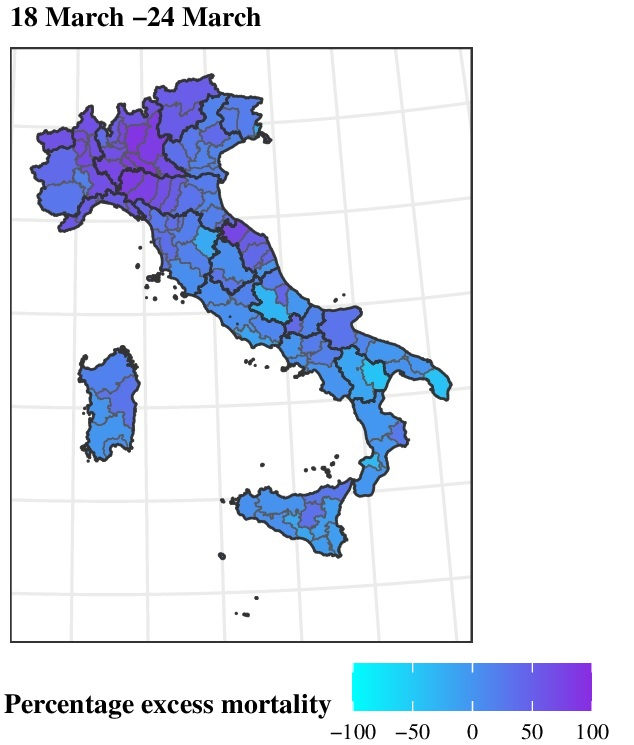
\includegraphics[scale=0.48]{Figures/Italy_Covid_March2020.jpg}
\caption{\footnotesize Map of the percent excess mortality for the 107 Italian provinces during the first wave of Covid-19 pandemic. Epidemiological week 18-24 March, 2020; males.}
\end{figure}
\end{frame}

\begin{frame}
\frametitle{Example of regular lattice data [3]}
\begin{figure}
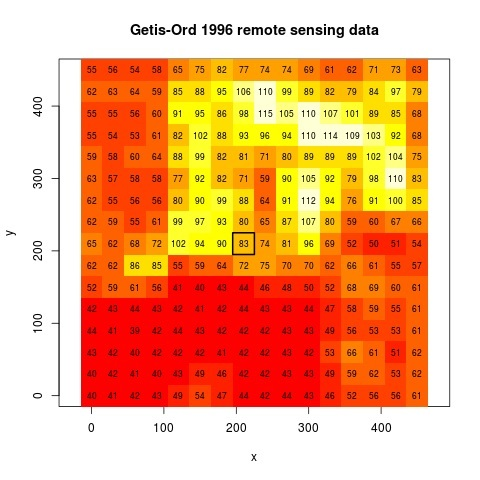
\includegraphics[scale=0.70]{Figures/Getis-Ord.jpg}
\caption{\footnotesize Regular lattice: Getis-Ord remote sensing example data (from package \texttt{spdep}).}
\end{figure}
\end{frame}

\begin{frame}
\frametitle{Example of geostatistical data [1]}
\begin{figure}
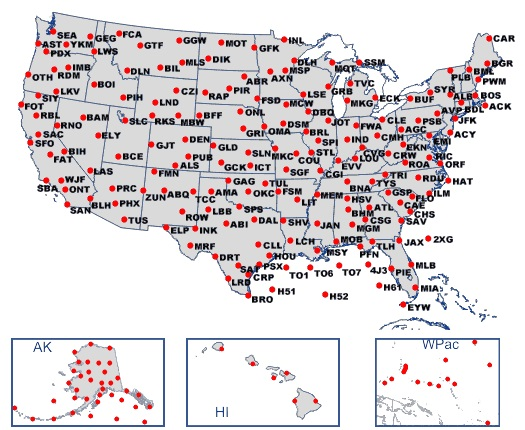
\includegraphics[scale=0.60]{Figures/Wind_Temp_StationsUS.jpg}
\caption{\footnotesize Map of wind and temperature stations in US (2019).}
\end{figure}
%\tiny{Source: \url{https://www.aviationweather.gov/windtemp}}
\footnotesize The data are gathered at a discrete set of points in an region of interest ($\mathcal{D}$), with the aim of understanding
the behaviour of an unobserved, spatially continuous phenomenon that exists throughout that region and could, in principle, be observed at any point in $\mathcal{D}$.
\end{frame}



\begin{frame}
\frametitle{Example of geostatistical data [2]}
\begin{figure}
\begin{center}
\begin{tabular}{cc}
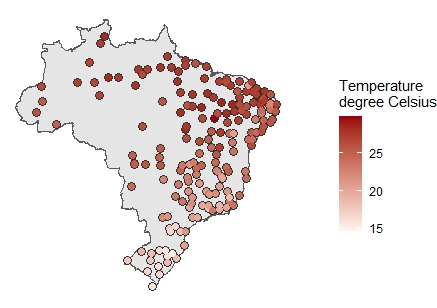
\includegraphics[width=6.5cm]{Rplot_Temp_Dry2018.jpeg}&
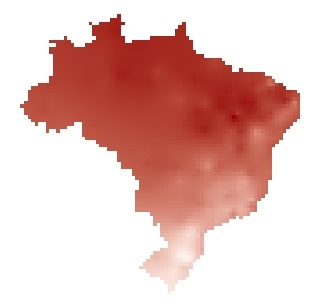
\includegraphics[width=4.3cm]{Rplot_Temp_Pred_Dry2018.jpeg}\\
Observed & Predicted \\
\end{tabular}
\end{center}
\footnotesize{\caption{Average air temperature in degree Celsius (March-November 2018)}}
\end{figure}
\footnotesize{We can reconstruct a surface from the finite set of observations taken at a finite number of spatial locations.}
\end{frame}

%\begin{frame}
%\frametitle{Example of geostatistical data [2]}
%\begin{figure}
%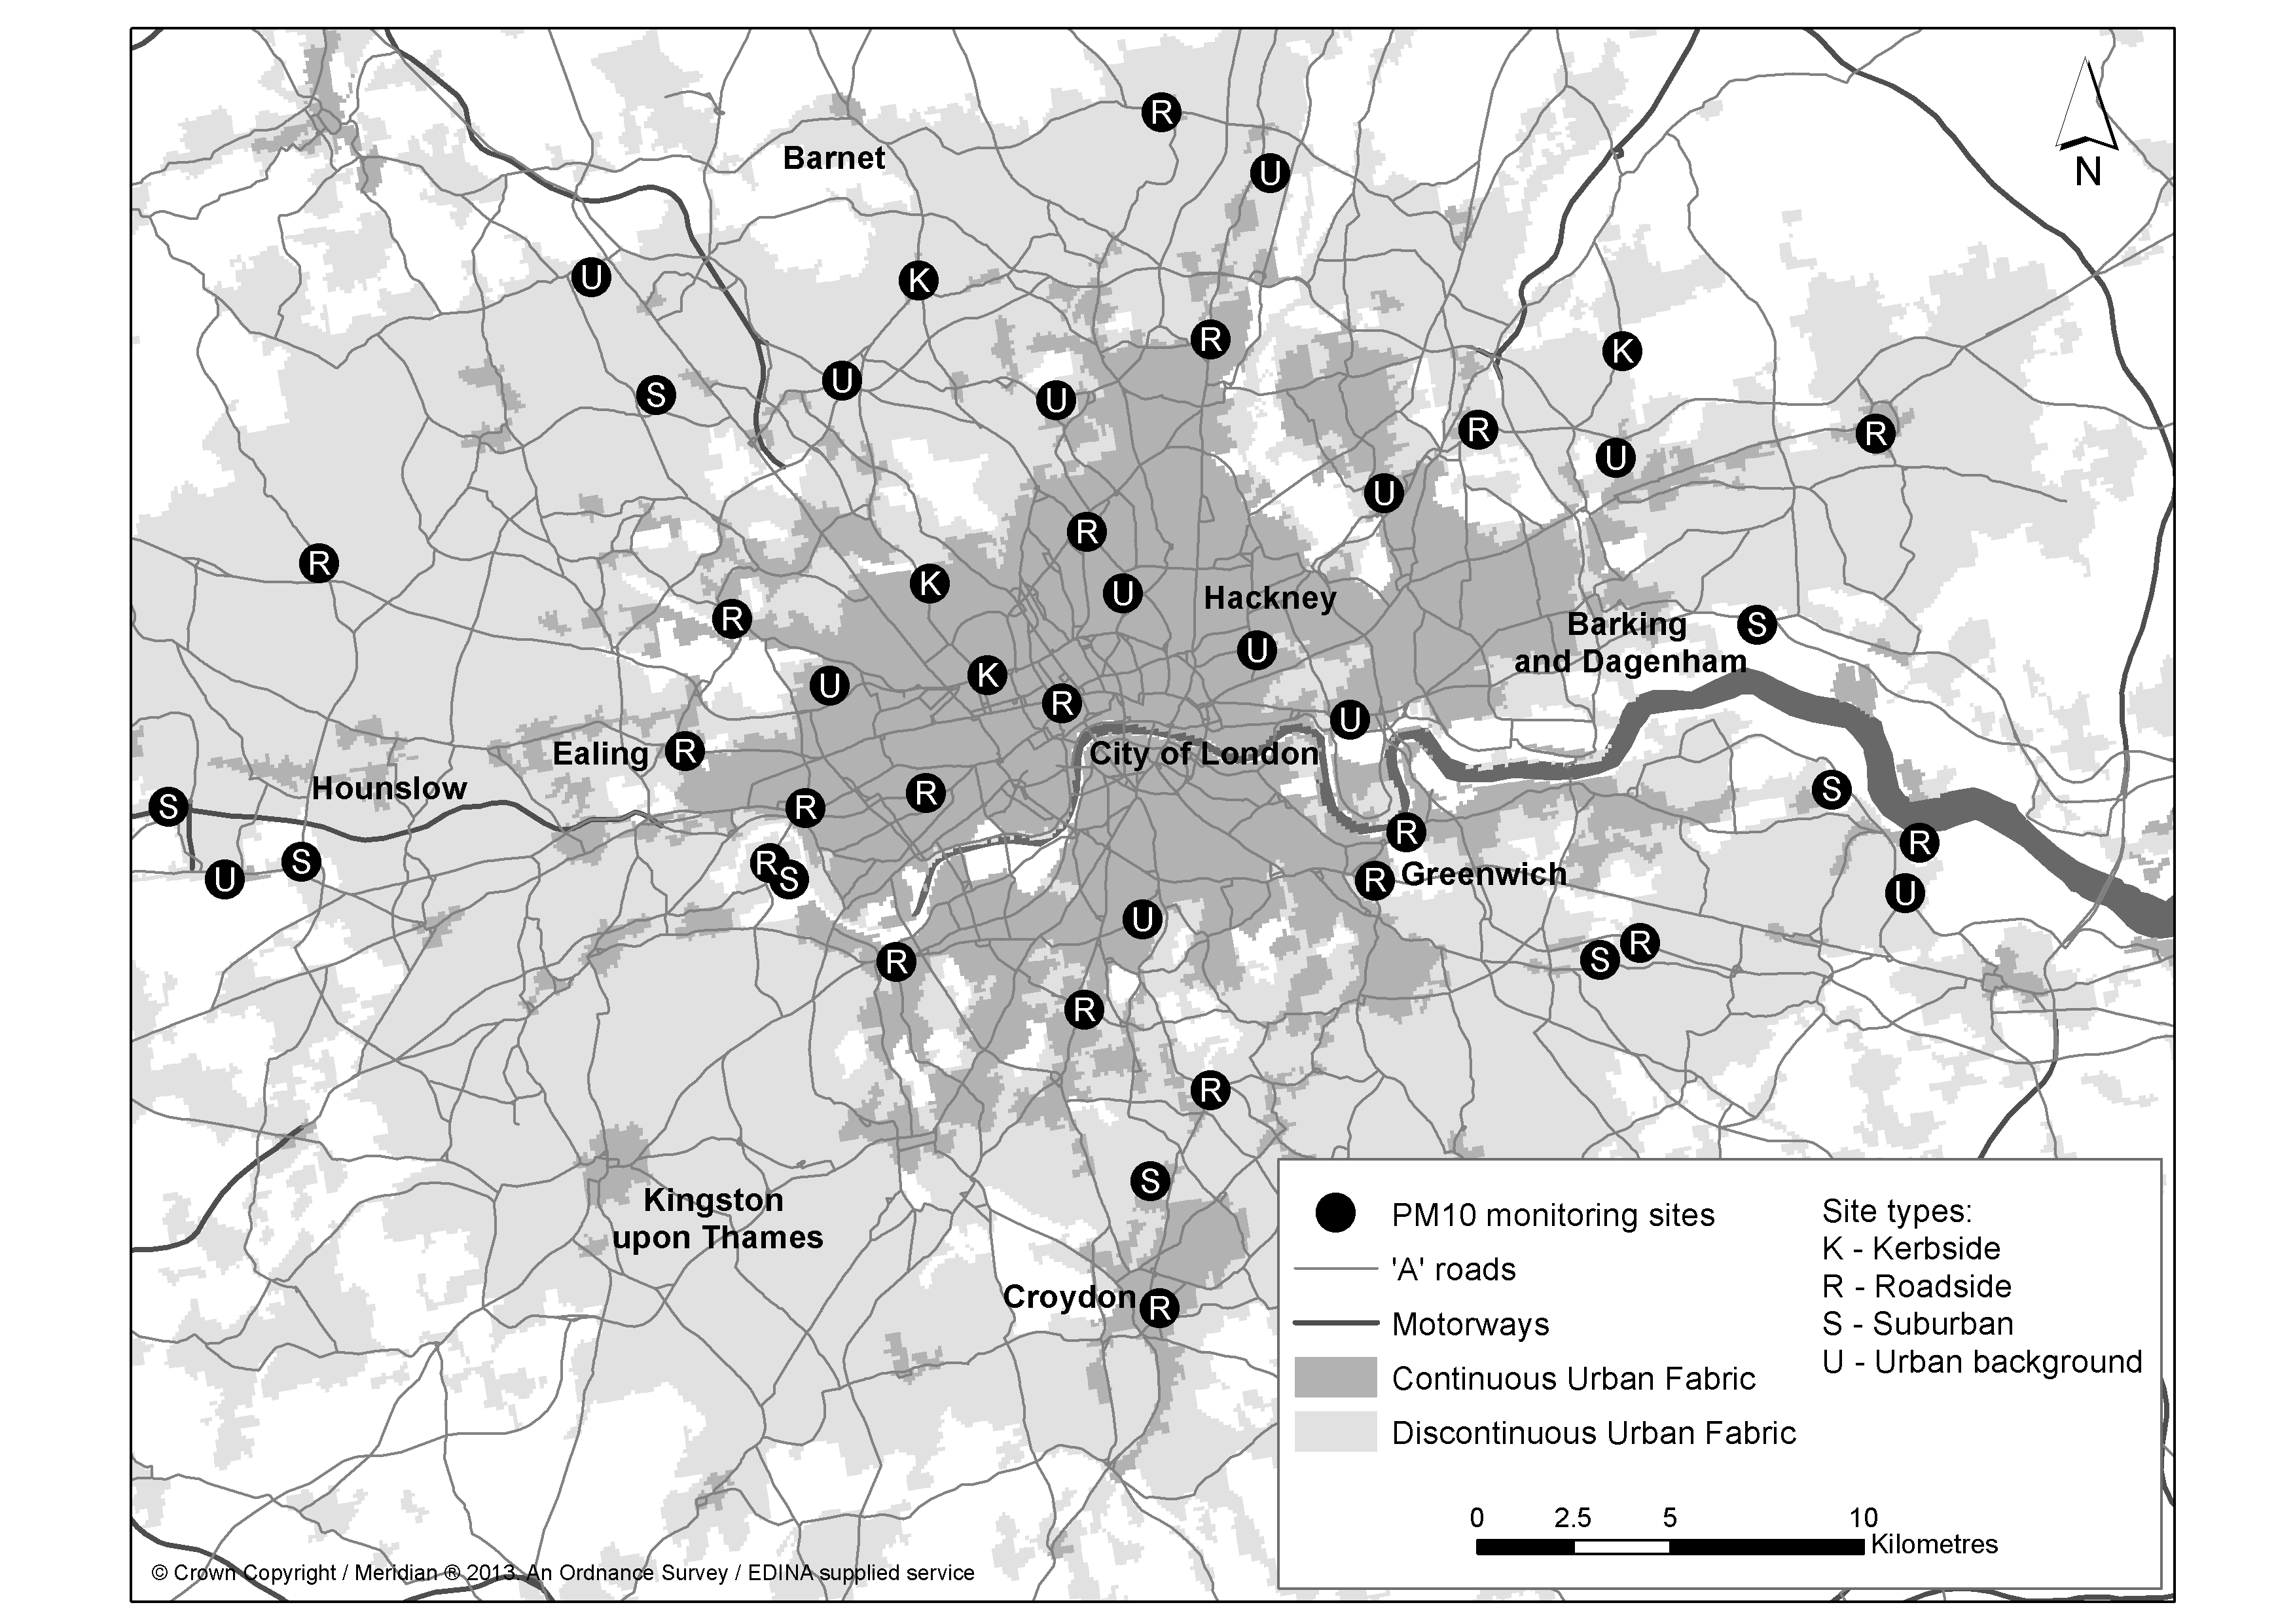
\includegraphics[scale=0.27]{Figures/MAP_PM10_GL.jpg}
%\caption{\footnotesize Location and siting characteristics of the air quality monitoring sites in Greater London for PM$_{10}$ (i.e. particulate %matter 10 micrometers or less in diameter).} %Source: \citet{Pirani2014}.}
%\end{figure}
%\end{frame}


\begin{frame}
\frametitle{Examples of point pattern data [1]}
%In point-pattern data, the locations themselves are stochastic.
\begin{figure}
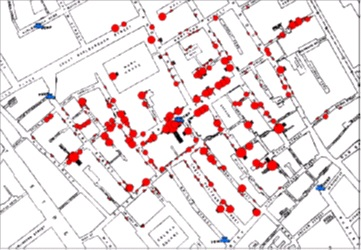
\includegraphics[scale=1]{Figures/colera.jpg}
\caption{\footnotesize John Snow's map of the 1854 London cholera outbreak}
\end{figure}
\footnotesize{In 1854, cholera hit the city of London. No one knew where the disease started. So, British physician John Snow started mapping the outbreak. \\
%It wasn’t just the disease. But he also mapped out roads, property boundaries, and water lines.
%When he added these features to a map, something interesting happened. He noticed that cholera cases were only along one water line. This was a breakthrough that connected geography to public health safety.
The question of primary interest is whether, and if so where and when, statistically unusual local concentrations of cases occur.}


%\begin{figure}
%\includegraphics[scale=0.70]{EarthQ.jpg}
%\caption{Location of earthquakes in north eastern Mediterranean region}
%\end{figure}
%Other examples in which points are the location of an \alert{event} of interest:
%\begin{itemize}
 % \item Location of crimes
 % \item Location of trees
 % \item Location of earthquakes
%\end{itemize}
\end{frame}


\begin{frame}
\frametitle{Examples of point pattern data [2]}
\begin{figure}
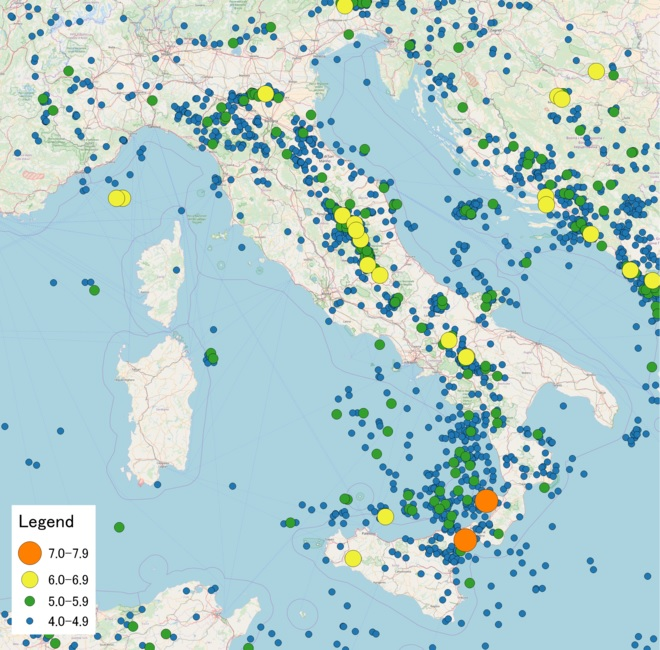
\includegraphics[scale=0.51]{Figures/Earthquakes_Italy.jpg}
\caption{\footnotesize Location of earthquakes in Italy 1900-2017 (moment magnitude scale). Source: Wikipedia.}
\end{figure}
%Other examples in which points are the location of an \alert{event} of interest:
%\begin{itemize}
 % \item Location of crimes
 % \item Location of trees
 % \item Location of earthquakes
%\end{itemize}
\end{frame}

\begin{frame}
\frametitle{Data we will work with}
In this module, we will work with:

\begin{itemize}
 \item Areal or lattice data
 \item Geostatistical or spatial-referenced data
 \end{itemize}
\end{frame}


%%%%%%%%%%%%%%%%%%%%%%%%%%%%%%%%%%%%%%%%%%%%%%%%%%%%%%%%%%%%%%%%
%%%%%%%%%%%%%%%%%%%%%%%%%%%%%%%%%%%%%%%%%%%%%%%%%%%%%%%%%%%%%%%%
%\subsection{Spatial data in R}

\begin{frame}
\frametitle{Spatial data in R: Vectors}
The are two fundamental distinctions: spatial \alert{vector} data and \alert{raster}.
\begin{itemize}
  \item \vfill \alert{Vector} represents the world using \alert{points}, \alert{lines} and \alert{polygons} or combinations of those, where:
      \begin{itemize}
      \item \vfill \emph{Point}, is a single point location, such as a geocoded address or a temperature sensor or the location of a bus stop;
      \item \vfill \emph{Line}, is a set of ordered points, connected by straight line segments such as route travel or connections between locations;
      \item \vfill \emph{Polygon}, is an area, marked by one or more enclosing lines such as local authority districts or census tracts.
      \end{itemize}
\end{itemize}
\end{frame}

\begin{frame}
Simple features, \texttt{sf} package \citep{Pebesma2018} support 17 geometry types. Of these, 7 are used in the vast majority of geographic research:
\begin{figure}
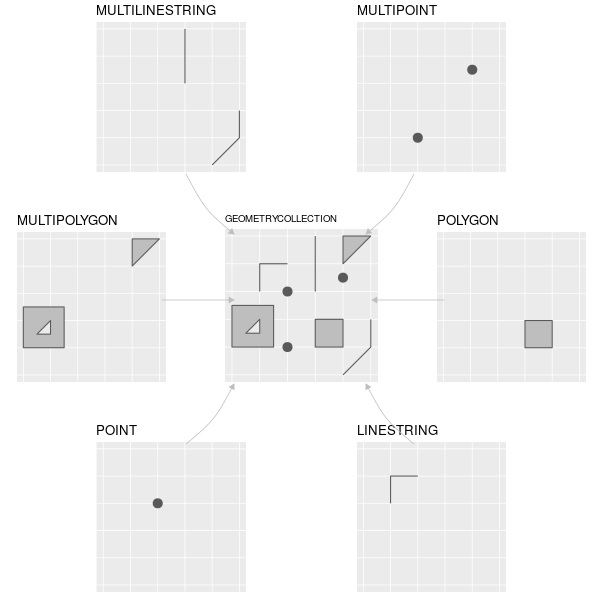
\includegraphics[scale=0.55]{Figures/Features_supported_by_sf.jpg}
\caption{\footnotesize Core geometry types supported by the R package sf. Source: \citet{Lovelace2019}; Section 2.2.}
\end{figure}
\end{frame}


\begin{frame}
\frametitle{Spatial data in R: Rasters}
\begin{itemize}
  \item \vfill \alert{Raster}: divides the surface into cells (also called pixels) of constant size. Each cell has a value associated with it, which might be numeric or categorical. 
   \begin{itemize}
   \item \vfill Raster maps usually represent continuous phenomena such as elevation, temperature, population density.
   \item \vfill Raster data are the basis of images used in web-mapping and have been a source of data since the origins of aerial photography and satellite-based remote sensing devices.
\end{itemize}
\end{itemize}
\end{frame}

\begin{frame}
Examples of continuous and categorical raster data. 
\begin{figure}
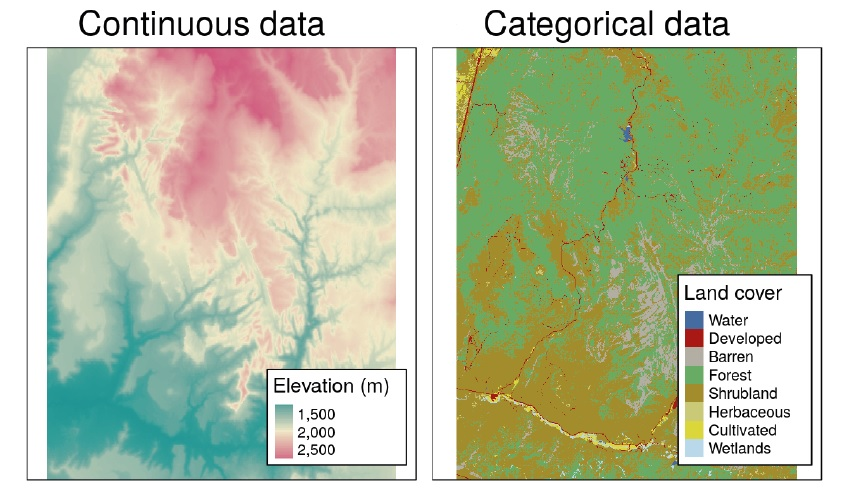
\includegraphics[scale=0.60]{Figures/Raster_data.jpg}
%\caption{\footnotesize Source: \citet[Section 2.3][]{Lovelace2019}.}
\end{figure} 

\footnotesize Source: \citet{Lovelace2019}; Section 2.3   
\end{frame}

\begin{frame}
\frametitle{Some R packages we will start to work with in week 6}
 \begin{footnotesize}
 \begin{itemize} \setlength\itemsep{\fill}
 \item  \texttt{sf}, which is a recently developed package for spatial vector data (points, lines, polygons etc.) and combines the functionality of three previous packages \texttt{sp}, \texttt{rgeos} and \texttt{rgdal}. It refers to a formal standard that describes how objects in the real world can be represented in computers, with emphasis on the spatial geometry of these objects
 \item  \texttt{sp}, which precedes \texttt{sf}, and with the \texttt{rgdal} and \texttt{rgeos} package, it creates a powerful tool to works with spatial data. Many R packages still depends on the \texttt{sp} package
 \item \texttt{spdep}, which includes functions and tests for evaluating spatial patterns and autocorrelation
 \item  \texttt{tidyverse}, which is a coherent system of packages for data manipulation, exploration and visualization
 \item \texttt{ggplot2}, \texttt{tmap} and \texttt{mapview} for visualization and maps
 \item \texttt{SpatialEpi}, which provides methods for spatial epidemiology
 \end{itemize}
 \end{footnotesize}
\end{frame}


\begin{frame}[fragile]

Many spatial R packages still depends on the \texttt{sp}, thus it is important to know how to convert \texttt{sp} to and from \texttt{sf} objects

{\scriptsize
\begin{verbatim}
library(spData); library(sf); library(tidyverse)

# world is a sf object containing a world map data
# from Natural Earth with a few variables from World Bank
world <- st_read(system.file("shapes/world.gpkg", package="spData"))
plot(world["pop"])                # plot world population

world_sp <- as(world, "Spatial")  # from sf to sp object
class(world_sp)                   # "SpatialPolygonsDataFrame"

world_sf <- st_as_sf(world_sp)    # from sp to sf object
class(world_sf)                   # "sf"  "data.frame"

\end{verbatim}
}
\vspace{-15pt}
\begin{figure}
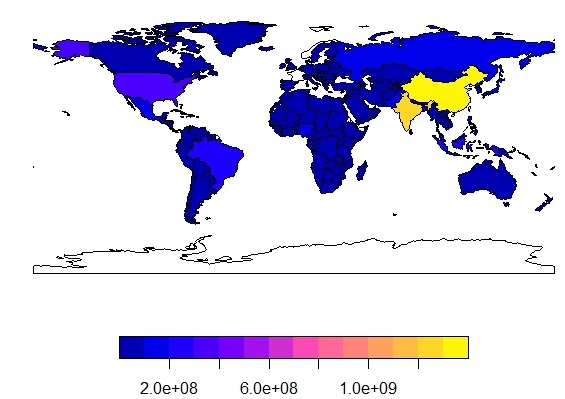
\includegraphics[scale=0.35]{World_pop.jpeg}
\end{figure}
\end{frame}


\begin{frame}[fragile]
\texttt{sf} works well with the \texttt{tidyverse} collection of R packages.\\
\vspace{5pt}
For example, functions can be combined using the pipe operator \scriptsize{$\%>\%$} \normalsize{(given that both packages are loaded)}
{\scriptsize
\begin{verbatim}
# Select and plot information for a single attribute
world %>% select(lifeExp) %>% plot()

\end{verbatim}
}
\begin{figure}
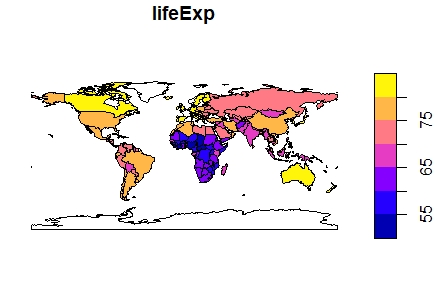
\includegraphics[scale=0.60]{LifeExp.jpeg}
\end{figure}
\end{frame}



\begin{frame}[fragile]
\texttt{sf} object includes spatial metadata like the coordinate reference
system (CRS), which are stored in a list column.\\
\vspace{5pt}
We can extract and plot only the geometry with the function $st\_geometry()$
{\scriptsize
\begin{verbatim}
# Extract geometry
worlg_geo <- st_geometry(world)

# Extract and plot out only the geometries
world %>% st_geometry() %>% plot()

\end{verbatim}
}
\vspace{-20pt}
\begin{figure}
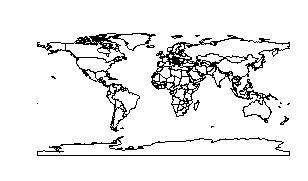
\includegraphics[scale=0.75]{World_geom.jpeg}
\end{figure}
\end{frame}


\begin{frame}
\frametitle{Articles and books cited in this lecture}
\footnotesize{
\bibliographystyle{asa}
\bibliography{refs}
}
\end{frame}

\end{document} 